\chapter{Température, entropie et énergie}

\lectureoverview{La température apparaît d’abord comme un facteur de conversion entre les unités des thermomètres usuels et les unités microscopiques d’énergie. Après avoir effectué la conversion correspondante de l’entropie thermodynamique en entropie statistique sans dimension, nous décrivons l’équilibre par une famille à un paramètre de distributions de probabilité. La dérivée \(dE/dS\) définit alors la température, et les deux premiers principes montrent pourquoi une différence de température détermine le sens du transfert d’énergie.}

\section{Facteurs de conversion et unités usuelles}

De nombreuses constantes physiques sont des facteurs de conversion. La vitesse de la lumière convertit une distance en durée :
\begin{equation}
 t=\frac{x}{c}.
\end{equation}
Si les distances et les durées sont mesurées dans des unités compatibles, on peut poser \(c=1\). Aucun effet physique ne disparaît : les deux types de mesure sont simplement exprimés sur une échelle commune.

La constante de Boltzmann joue le même rôle. Elle convertit la température indiquée par un thermomètre à \emph{échelle humaine} en énergie. Cette précision est importante. Ces unités sont choisies parce que les instruments macroscopiques permettent de les produire et de les distinguer, et non parce que la dynamique microscopique les privilégie.

Le degré Celsius a été défini en divisant en cent parties l’intervalle entre les points de congélation et d’ébullition de l’eau à la pression normale. Le kelvin utilise un degré de même amplitude, mais fixe le zéro au zéro absolu. Choisir une autre substance, un autre intervalle ou des degrés Fahrenheit modifierait les nombres, mais pas la physique.

\begin{classroomqa}
\audiencequestion{L’échelle Fahrenheit était-elle déjà une construction du XVIIe siècle ?}
\lecturerresponse{La date précise n’est pas nécessaire ici. L’essentiel est que toutes ces échelles ont été conçues à partir de températures que l’on pouvait produire et mesurer. L’amplitude du degré est conventionnelle, et non déterminée par la physique microscopique.
\lecturetimestamp{00:01:34--00:01:50}}
\end{classroomqa}

À l’époque où ces échelles ont été créées, l’origine moléculaire de la chaleur n’était pas accessible à l’expérimentation. On pouvait observer une variation d’un degré avec un thermomètre macroscopique, tandis qu’il était impossible de mesurer l’énergie d’une molécule. Il était donc naturel d’inventer une unité de température avant de savoir que la température est fondamentalement une échelle d’énergie.

\section{Pourquoi la température s’exprime en unités d’énergie}

Considérons un gaz monoatomique dilué. Ici, « dilué » signifie que l’on peut négliger, pour l’instant, les énergies d’interaction entre les molécules. À l’équilibre thermique, l’équipartition attribue \(T_{\mathrm K}/2\) fois la constante de Boltzmann à chaque degré de liberté de translation quadratique. Dans trois dimensions spatiales,
\begin{equation}
 \left\langle E_{\mathrm{kin}}\right\rangle
 =\frac{3}{2}k_{\mathrm B}T_{\mathrm K}.
 \label{eq:sm2-equipartition-kelvin}
\end{equation}
Le facteur trois compte les mouvements selon les directions \(x\), \(y\) et \(z\). Le facteur un demi provient de l’énergie cinétique quadratique.

Cette relation n’est pas propre à une seule espèce moléculaire. Dans un mélange d’hélium et d’oxygène à l’équilibre, chaque particule en translation libre possède la même énergie cinétique moyenne du centre de masse, même si les particules les plus lourdes se déplacent plus lentement. Puisque
\begin{equation}
 E_{\mathrm{kin}}=\frac{1}{2}mv^2,
\end{equation}
l’égalité des énergies caractéristiques implique \(v\propto m^{-1/2}\).

On peut pousser la même idée jusqu’à un exemple volontairement extrême. Suspendons une boule de bowling dans un fluide et laissons le système complet atteindre l’équilibre. Ses degrés de liberté de translation brownienne sont régis par la même échelle d’énergie que ceux d’une molécule. La vitesse de la boule est extraordinairement plus faible parce que sa masse est extraordinairement plus grande ; mais la température compare des échelles d’énergie, et non des vitesses.

À température ambiante, \(T_{\mathrm K}\) vaut environ \(300\,\mathrm K\), alors que l’énergie d’un degré de liberté microscopique est infime en joules. Le facteur de conversion est donc très petit :
\begin{equation}
 k_{\mathrm B}\simeq 1.38\times10^{-23}\,
 \mathrm{J\,K^{-1}}.
 \label{eq:sm2-boltzmann-value}
\end{equation}
Son ordre de grandeur et le nombre d’Avogadro sont liés, et non fortuitement similaires :
\begin{equation}
 R=N_{\mathrm A}k_{\mathrm B}.
\end{equation}
La constante des gaz \(R\) décrit une mole, tandis que \(k_{\mathrm B}\) décrit l’échelle correspondante par constituant microscopique.

Les formules fondamentales contiennent fréquemment la combinaison \(k_{\mathrm B}T_{\mathrm K}\). Il est donc plus commode de définir
\begin{equation}
 T\equiv k_{\mathrm B}T_{\mathrm K}.
 \label{eq:sm2-energy-temperature}
\end{equation}
Désormais, \(T\) a lui-même les unités d’une énergie, et
\eqref{eq:sm2-equipartition-kelvin} devient
\begin{equation}
 \left\langle E_{\mathrm{kin}}\right\rangle=\frac{3}{2}T.
 \label{eq:sm2-equipartition-natural}
\end{equation}
Si l’énergie est mesurée en joules, la température l’est en joules. Si l’énergie est mesurée en électronvolts, la température l’est en électronvolts. Il n’existe pas de nouvelle unité naturelle appelée unité de température.

\section{Deux conventions pour l’entropie}

La même conversion intervient du côté de l’entropie. La thermodynamique macroscopique est née de l’étude des machines thermiques. Carnot a fourni le raisonnement décisif sur ces machines ; Clausius a ensuite introduit l’entropie thermodynamique et le symbole \(S\). Dans les notations utilisées ici, appelons cette grandeur macroscopique \(S_{\mathrm C}\). Elle s’exprime en énergie divisée par la température indiquée par un thermomètre, par exemple en joules par kelvin.

L’entropie statistique est sans dimension. Pour une distribution discrète,
\begin{equation}
 S=-\sum_i p_i\log p_i.
 \label{eq:sm2-statistical-entropy}
\end{equation}
Avec les logarithmes népériens, une alternative binaire équiprobable a une entropie de \(\log2\) ; avec les logarithmes en base deux, cette même quantité est appelée un bit. Les deux conventions de l’entropie sont liées par
\begin{equation}
 S=\frac{S_{\mathrm C}}{k_{\mathrm B}},
 \qquad
 S_{\mathrm C}=k_{\mathrm B}S.
 \label{eq:sm2-entropy-conversion}
\end{equation}
Une valeur macroscopique modeste en \(\mathrm{J\,K^{-1}}\) correspond à une entropie sans dimension énorme, car elle dénombre l’information répartie entre un nombre immense de constituants microscopiques.

Les équations \eqref{eq:sm2-energy-temperature} et
\eqref{eq:sm2-entropy-conversion} fixent la convention utilisée dans tout ce qui suit :
\[
 [T]=[\text{energy}],
 \qquad
 [S]=1.
\]
La constante de Boltzmann peut désormais disparaître des formules de travail. On peut toujours la réintroduire en remplaçant \(T\) par \(k_{\mathrm B}T_{\mathrm K}\) et \(S\) par \(S_{\mathrm C}/k_{\mathrm B}\).

\begin{classroomqa}
\audiencequestion{À part le facteur \(3/2\), la nouvelle température est-elle simplement une énergie mesurée en joules ?}
\lecturerresponse{Oui, si l’on choisit le joule comme unité d’énergie. Le joule est l’unité MKS \(\mathrm{kg\,m^2\,s^{-2}}\). On pourrait aussi utiliser les électronvolts ou toute autre unité d’énergie ; la température devrait alors être exprimée dans cette même unité. Le facteur \(3/2\) appartient à l’exemple du gaz parfait, et non à la définition de la température.
\lecturetimestamp{00:15:49--00:16:45}}
\end{classroomqa}

\begin{classroomqa}
\audiencequestion{Si le tableau indique des kelvins, \(k_{\mathrm B}\) n’est-elle pas alors une constante bien définie ?}
\lecturerresponse{Elle est bien définie une fois spécifiées les unités de température et d’énergie. Si l’on remplace le kelvin par le degré Fahrenheit, ou le joule par l’électronvolt, sa valeur numérique change. C’est précisément ainsi que se comporte un facteur de conversion.
\lecturetimestamp{00:16:46--00:18:33}}
\end{classroomqa}

\begin{classroomqa}
\audiencequestion{La valeur numérique de la constante de Boltzmann est-elle déterminée expérimentalement ?}
\lecturerresponse{Oui. Historiquement, son évaluation nécessitait des informations microscopiques sur les atomes et leur densité numérique. Boltzmann avait compris le lien entre l’énergie moléculaire et la température avant que ces grandeurs soient connues avec précision, un peu comme Newton connaissait le rôle de la constante gravitationnelle avant qu’elle soit mesurée avec exactitude.
\lecturetimestamp{00:18:46--00:20:00}}
\end{classroomqa}

\section{L’équilibre est un état statistique}

La conversion des unités n’a toujours pas défini la température. Toucher un objet chaud donne une intuition biologique utile, mais la température est une grandeur physique dérivée, construite à partir de l’énergie et de l’entropie.

Imaginons un système en contact avec un grand environnement dont les conditions macroscopiques sont fixées. De l’énergie peut passer de l’un à l’autre. Si le système possède initialement trop d’énergie, il en perd en moyenne ; s’il n’en a pas assez, il en gagne en moyenne. À l’équilibre thermique, les échanges microscopiques se poursuivent, mais il n’y a aucun flux moyen net dans un sens ou dans l’autre.

Notons \(i\) un état microscopique exact du système et \(E_i\) l’énergie de cet état. L’équilibre ne signifie pas que le système reste figé dans un état unique. Son interaction avec l’environnement modifie continuellement son état microscopique ; nous attribuons donc une probabilité \(P_i\) à chaque possibilité. Les relations de base sont
\begin{align}
 \sum_i P_i &=1,
 \label{eq:sm2-normalization}\\
 \sum_i P_iE_i &=\overline E,
 \label{eq:sm2-mean-energy}\\
 S&=-\sum_iP_i\log P_i.
 \label{eq:sm2-equilibrium-entropy}
\end{align}
La barre sur \(\overline E\) souligne que l’énergie du sous-système fluctue. Une mesure peut donner une valeur et la suivante une autre ; des mesures répétées suivent la distribution dont la moyenne est
\eqref{eq:sm2-mean-energy}.

\begin{figure}[t]
\centering
\includegraphics[width=0.82\textwidth]{lecture_02_figure_02.png}
\caption{Normalisation et énergie moyenne au tableau :
\(\sum_iP(i)=1\) et \(\sum_iP(i)E(i)=\langle E\rangle\).}
\lectureframe{00:24:10}
\end{figure}

\section{Une famille indexée par l’énergie moyenne}

La distribution d’équilibre dépend fortement de l’énergie moyenne. Posons une casserole d’eau sur le feu : \(\overline E\) augmente ; mettons-la dans la neige : \(\overline E\) diminue. Les probabilités varient avec elle. Il faut donc considérer l’équilibre non comme une distribution unique, mais comme une famille à un paramètre :
\begin{equation}
 P_i(\overline E).
 \label{eq:sm2-family}
\end{equation}
Chaque élément de cette famille vérifie
\begin{align}
 \sum_iP_i(\overline E)&=1,
 \label{eq:sm2-family-normalization}\\
 \sum_iP_i(\overline E)E_i&=\overline E.
 \label{eq:sm2-family-mean}
\end{align}

\begin{figure}[t]
\centering
\includegraphics[width=0.88\textwidth]{lecture_02_figure_03.png}
\caption{Transition vers \(P(i,\overline E)\). Les équations précédentes de normalisation, d’énergie moyenne et d’entropie restent visibles tandis que la famille de distributions est introduite.}
\lectureframe{00:26:29}
\end{figure}

Pour un graphique schématique, classons les états par ordre croissant de \(E_i\). L’axe horizontal peut alors représenter soit l’indice \(i\), soit l’énergie correspondante. Lorsque l’énergie moyenne augmente, le poids des probabilités se déplace vers les états situés plus à droite. L’aire totale sous chaque courbe doit rester égale à l’unité.

\begin{figure}[t]
\centering
\includegraphics[width=0.88\textwidth]{lecture_02_figure_04.png}
\caption{Plusieurs distributions schématiques \(P(i,\overline E)\). Les courbes dont le poids se répartit davantage vers la droite ont une énergie moyenne plus élevée, tout en restant chacune normalisée.}
\lectureframe{00:28:40}
\end{figure}

\begin{figure}[t]
\centering
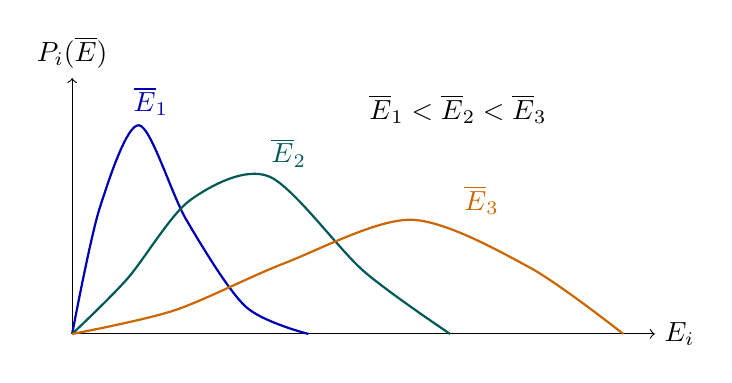
\begin{tikzpicture}[x=1cm,y=1cm]
\draw[->] (0,0) -- (7.4,0) node[right] {$E_i$};
\draw[->] (0,0) -- (0,3.25) node[above] {$P_i(\overline E)$};
\draw[thick,blue!70!black]
  plot[smooth] coordinates {(0,0) (0.35,1.6) (0.85,2.65) (1.45,1.45)
  (2.2,0.35) (3.0,0)};
\draw[thick,teal!70!black]
  plot[smooth] coordinates {(0,0) (0.7,0.7) (1.5,1.7) (2.5,2.0)
  (3.7,0.8) (4.8,0)};
\draw[thick,orange!80!black]
  plot[smooth] coordinates {(0,0) (1.3,0.3) (2.7,0.9) (4.3,1.45)
  (5.8,0.85) (7.0,0)};
\node[blue!70!black] at (1.0,2.95) {\(\overline E_1\)};
\node[teal!70!black] at (2.75,2.3) {\(\overline E_2\)};
\node[orange!80!black] at (5.2,1.7) {\(\overline E_3\)};
\node at (4.9,2.85) {\(\overline E_1<\overline E_2<\overline E_3\)};
\end{tikzpicture}
\caption{Version au propre du schéma au tableau. Les courbes n’ont pas besoin d’avoir ces formes précises ; seules leur normalisation et l’ordre de leurs énergies moyennes sont utilisés.}
\end{figure}

\begin{classroomqa}
\audiencequestion{La notation est-elle circulaire ? L’énergie moyenne est calculée à partir de la distribution, alors que la distribution est indexée par l’énergie moyenne.}
\lecturerresponse{Commençons par une famille à un paramètre de distributions d’équilibre choisies empiriquement. Chaque élément possède une énergie moyenne. Si les moyennes des différents éléments sont distinctes, on peut utiliser cette moyenne comme paramètre pour indexer la famille. Cette notation ne permet pas encore de déduire la famille ; la distribution de Boltzmann en fournira la dérivation plus tard.
\lecturetimestamp{00:28:35--00:29:44}}
\end{classroomqa}

\begin{classroomqa}
\audiencequestion{Pourquoi parler d’énergie moyenne plutôt que d’énergie totale ?}
\lecturerresponse{Le sous-système échange de l’énergie avec un bain thermique, par exemple l’atmosphère qui entoure un récipient de gaz aux parois perméables à la chaleur. Son énergie instantanée fluctue. De nombreuses mesures produisent une distribution, et \(\overline E\) est la moyenne de ces résultats. L’énergie du système fermé plus vaste, constitué du sous-système et du bain, peut néanmoins rester fixée.
\lecturetimestamp{00:29:46--00:30:56}}
\end{classroomqa}

\begin{classroomqa}
\audiencequestion{Des états microscopiques différents peuvent-ils avoir la même énergie, et des distributions différentes la même énergie moyenne ?}
\lecturerresponse{Les deux cas sont possibles. La contrainte sur l’énergie moyenne autorise à elle seule de nombreuses distributions ; il faut donc un argument physique supplémentaire pour justifier la famille d’équilibre particulière à un paramètre. Son origine et sa forme de Boltzmann seront dérivées plus tard. L’égalité des énergies d’états microscopiques distincts est une question distincte, appelée dégénérescence.
\lecturetimestamp{00:30:58--00:32:22}}
\end{classroomqa}

\subsection{Étiquettes des états, dégénérescence et corrélation}

Il faut distinguer plusieurs notions qu’il est facile de confondre.

Premièrement, de nombreuses distributions de probabilité peuvent avoir la même énergie moyenne. La famille d’équilibre à un paramètre ne découle pas de la seule contrainte sur l’énergie moyenne. C’est la famille particulière sélectionnée par l’équilibration ; sa forme sera identifiée plus tard comme la distribution de Boltzmann.

Deuxièmement, plusieurs états microscopiques distincts peuvent avoir la même énergie. On parle alors de dégénérescence. Dans la discussion au tableau, on néglige provisoirement les dégénérescences exactes afin de pouvoir classer sans ambiguïté les états par énergie. La dégénérescence est en fait fréquente dans les systèmes qui possèdent des symétries, mais elle ne pose aucune difficulté conceptuelle : conservons l’étiquette d’état \(i\), autorisons des valeurs répétées de \(E_i\) et sommons sur tous les états.

Troisièmement, la corrélation n’est pas un autre terme pour désigner la dégénérescence. La corrélation concerne une distribution conjointe de deux grandeurs aléatoires et demande si la connaissance de l’une modifie les probabilités de l’autre. Les étiquettes mutuellement exclusives \(i\) et \(j\) dans une même liste d’états microscopiques ne sont pas, à elles seules, deux variables aléatoires dont on calcule la corrélation.

\begin{classroomqa}
\audiencequestion{La construction suppose-t-elle que les différents états \(i\) sont indépendants, et que se passe-t-il si deux d’entre eux sont corrélés ?}
\lecturerresponse{Une étiquette d’état est une valeur possible d’une seule variable aléatoire microscopique. L’indépendance et la corrélation nécessitent deux variables distribuées conjointement ; ces termes ne s’appliquent donc pas directement à deux étiquettes possibles de cette liste. L’égalité des énergies d’états distincts relève plutôt de la dégénérescence.
\lecturetimestamp{00:32:23--00:33:22}}
\end{classroomqa}

\begin{classroomqa}
\audiencequestion{Que se passe-t-il si deux états distincts ont exactement la même énergie ?}
\lecturerresponse{C’est le cas de la dégénérescence. Pour le graphique présenté maintenant, nous adoptons l’hypothèse simplificatrice qu’aucune énergie ne coïncide avec une autre, et classons les états par ordre croissant d’énergie. Les formules de probabilité utilisées plus tard ne nécessitent pas cette hypothèse : il suffit de compter séparément les états dégénérés.
\lecturetimestamp{00:33:23--00:34:04}}
\end{classroomqa}

\begin{classroomqa}
\audiencequestion{La signification de l’indice \(i\) est-elle arbitraire ?}
\lecturerresponse{Les états microscopiques eux-mêmes ne sont pas arbitraires : chacun spécifie toutes les positions, les quantités de mouvement ou les autres données nécessaires à une description exacte. Seuls leurs noms sont arbitraires ; pour le schéma, nous choisissons donc des étiquettes dans l’ordre croissant des énergies.
\lecturetimestamp{00:34:06--00:35:15}}
\end{classroomqa}

\section{L’entropie devient une fonction de l’énergie}

Chaque élément de la famille d’équilibre possède une entropie. En substituant \eqref{eq:sm2-family} dans \eqref{eq:sm2-equilibrium-entropy}, on obtient
\begin{equation}
 S(\overline E)
 =-\sum_iP_i(\overline E)\log P_i(\overline E).
 \label{eq:sm2-entropy-energy}
\end{equation}
Il ne s’agit pas d’une fonction universelle commune à tous les systèmes physiques. Elle dépend du spectre du système et de sa famille d’équilibre. Une fois cette famille spécifiée, l’énergie et l’entropie sont toutefois liées : lorsqu’on parcourt la famille, les deux varient.

Dans les systèmes ordinaires, la probabilité se répartit généralement sur davantage d’états lorsque l’énergie moyenne augmente ; \(S\) augmente donc habituellement avec \(\overline E\). Pour l’instant, supposons que cette relation soit régulière et localement inversible. Les exceptions sont importantes, mais le cas simple permet d’exposer la définition dont nous avons besoin.

\section{La dérivée qui définit la température}

Posons une question concrète : de combien l’énergie moyenne doit-elle varier pour que l’entropie augmente d’une alternative binaire ? En unités logarithmiques naturelles, cette variation d’entropie vaut \(\log2\).

Pour des éléments voisins d’une famille régulière,
\begin{equation}
 dE=\frac{dE}{dS}\,dS.
 \label{eq:sm2-differential-identity}
\end{equation}
À ce stade, l’équation n’est qu’une application de la règle de dérivation en chaîne. Son coefficient possède cependant exactement les dimensions et le rôle physique requis pour la température.

\begin{definition}La température exprimée en unités d’énergie est définie par
\begin{equation}
 T\equiv\frac{dE}{dS}.
 \label{eq:sm2-temperature-definition}
\end{equation}
De manière équivalente,
\begin{equation}
 dE=T\,dS,
 \qquad
 dS=\frac{1}{T}\,dE.
 \label{eq:sm2-fundamental-differentials}
\end{equation}
\end{definition}

Pour une variation suffisamment petite d’un bit,
\begin{equation}
 \Delta E\simeq T\log2.
 \label{eq:sm2-one-bit-energy}
\end{equation}
La référence à un bit sert uniquement à rendre la dérivée concrète. La même relation locale vaut pour toute variation d’entropie suffisamment petite.

\begin{classroomqa}
\audiencequestion{Puisque l’entropie a été écrite \(S(E)\), \(dS/dE\) ne serait-elle pas la dérivée la plus naturelle ?}
\lecturerresponse{Les deux dérivées contiennent la même information lorsque la relation est localement inversible :
\[
 \frac{dE}{dS}=\left(\frac{dS}{dE}\right)^{-1}.
\]
Par convention, la température est \(dE/dS\), tandis que l’inverse de la température est \(dS/dE=1/T\).
\lecturetimestamp{00:40:24--00:40:54}}
\end{classroomqa}

Ici, une seule variable thermodynamique varie ; les dérivées ordinaires suffisent donc. Si le volume, le nombre de particules, l’aimantation ou d’autres variables peuvent varier, il faut utiliser des dérivées partielles et préciser quelles grandeurs sont maintenues constantes. La définition présente correspond à une coupe à une variable de cette géométrie thermodynamique plus générale.

\subsection{Pourquoi la constante de Boltzmann s’élimine}

Revenons brièvement aux unités des thermomètres. En utilisant
\[
 T=k_{\mathrm B}T_{\mathrm K},
 \qquad
 S=\frac{S_{\mathrm C}}{k_{\mathrm B}},
\]
la relation fondamentale devient
\begin{align}
 dE
 &=\bigl(k_{\mathrm B}T_{\mathrm K}\bigr)
   d\left(\frac{S_{\mathrm C}}{k_{\mathrm B}}\right)\\
 &=T_{\mathrm K}\,dS_{\mathrm C}.
 \label{eq:sm2-carnot-form}
\end{align}
Un facteur \(k_{\mathrm B}\) intervient par la température et le facteur réciproque par l’entropie. Ils s’éliminent. C’est pourquoi un manuel de thermodynamique conventionnel peut écrire \eqref{eq:sm2-carnot-form} sans faire apparaître la constante de Boltzmann.

\begin{classroomqa}
\audiencequestion{La relation \(S(E)\) doit-elle être inversible ?}
\lecturerresponse{Pas toujours. Pour les systèmes ordinaires dans le régime considéré ici, une énergie croissante élargit généralement la distribution d’équilibre et augmente l’entropie ; \(S(E)\) est donc monotone et \(T>0\). Les systèmes à spectre borné peuvent fournir des contre-exemples, notamment des régimes où l’entropie diminue avec l’énergie et où la température statistique est négative. Nous laissons ces cas de côté pour l’instant.
\lecturetimestamp{00:44:30--00:45:57}}
\end{classroomqa}

\section{De la dérivée abstraite aux notions de chaud et de froid}

La définition par une dérivée est universelle, mais reste abstraite. Nous voulons retrouver l’énoncé familier selon lequel l’énergie s’écoule d’un corps plus chaud vers un corps plus froid. La douleur causée par le contact avec une surface chaude relève de la biologie ; la couleur et le rayonnement émis dépendent des propriétés de la lumière. Une définition statistique doit aussi s’appliquer à un gaz idéalisé, même si l’on néglige le rayonnement.

\begin{classroomqa}
\audiencequestion{Le rayonnement émis par un objet chaud pourrait-il fournir la définition fondamentale de la température ?}
\lecturerresponse{Le rayonnement constitue un thermomètre utile, mais il fait intervenir la physique de la lumière. La mécanique statistique doit définir la température pour des systèmes tels qu’une boîte de gaz, sans dépendre de propriétés optiques. Le sens des échanges d’énergie est un critère plus général.
\lecturetimestamp{00:46:42--00:47:20}}
\end{classroomqa}

Préparons deux systèmes \(A\) et \(B\), chacun initialement à l’équilibre, à des températures \(T_A\) et \(T_B\). Ils sont d’abord isolés l’un de l’autre. Mettons-les ensuite en contact thermique faible : le \emph{tube mince} permet à de petites quantités d’énergie de passer dans les deux sens sans détruire l’identité de chacun des deux sous-systèmes.

\begin{figure}[t]
\centering
\includegraphics[width=0.88\textwidth]{lecture_02_figure_05.png}
\caption{Les systèmes \(A\) et \(B\), préparés séparément et caractérisés par les températures \(T_A\) et \(T_B\), juste avant l’examen d’un contact thermique faible.}
\lectureframe{00:48:55}
\end{figure}

\begin{figure}[t]
\centering
\begin{tikzpicture}[>=Stealth]
\draw[rounded corners,thick,fill=blue!6] (0,0) rectangle (2.6,2.4);
\draw[rounded corners,thick,fill=orange!8] (5.4,0) rectangle (8,2.4);
\draw[thick] (2.6,1.35) -- (5.4,1.35);
\draw[thick] (2.6,1.05) -- (5.4,1.05);
\draw[<->,very thick] (3.15,1.2) -- (4.85,1.2)
  node[midway,above] {\(\delta E\)};
\node at (1.3,1.45) {\Large \(A\)};
\node at (6.7,1.45) {\Large \(B\)};
\node at (1.3,0.65) {\(T_A,S_A,E_A\)};
\node at (6.7,0.65) {\(T_B,S_B,E_B\)};
\node at (4,0.35) {\small weak thermal contact};
\end{tikzpicture}
\caption{L’énergie fluctue à travers le contact faible, tandis que le système combiné reste isolé.}
\end{figure}

Supposons, sans perte de généralité, que
\begin{equation}
 T_B>T_A.
 \label{eq:sm2-temperature-order}
\end{equation}
L’expérience indique que \(B\) devrait perdre de l’énergie et que \(A\) devrait en gagner. Trois faits permettent de transformer cette attente en calcul.

\subsection{Additivité de l’entropie}

Pour deux sous-systèmes faiblement couplés, dont les possibilités microscopiques se combinent indépendamment, le nombre de possibilités conjointes est le produit des nombres de possibilités :
\[
 W_{AB}=W_AW_B.
\]
L’entropie étant logarithmique,
\begin{equation}
 S_{\mathrm{tot}}=S_A+S_B.
 \label{eq:sm2-entropy-additivity}
\end{equation}
On obtient le même résultat directement à partir de l’entropie de Shannon d’une distribution produit.

\begin{classroomqa}
\classquestion{Pourquoi l’entropie du système combiné est-elle additive ?}
\lecturerresponse{Parce que le nombre de possibilités sous-jacent se multiplie, tandis que l’entropie fait intervenir un logarithme :
\(\log(W_AW_B)=\log W_A+\log W_B\). La faiblesse de l’interaction permet de décrire les sous-systèmes et justifie cette forme additive au premier ordre.
\lecturetimestamp{00:51:06--00:52:03}}
\end{classroomqa}

\subsection{Les premier et deuxième principes}

Le système combiné est isolé, donc l’énergie échangée à l’intérieur est conservée :
\begin{equation}
 dE_A+dE_B=0,
 \qquad
 dE_B=-dE_A.
 \label{eq:sm2-first-law}
\end{equation}
C’est le premier principe dans le cadre de cette expérience.

Nous posons ici le deuxième principe comme un postulat, qui sera expliqué plus en profondeur par la suite. Lorsque les systèmes mis en contact évoluent spontanément vers leur nouvel équilibre,
\begin{equation}
 dS_{\mathrm{tot}}=dS_A+dS_B\geq0.
 \label{eq:sm2-second-law}
\end{equation}
L’inégalité stricte décrit l’évolution spontanée qui éloigne de l’équilibre ; à l’équilibre, l’égalité vaut pour une variation réversible au premier ordre.

Enfin, la définition de la température s’applique à chacun des sous-systèmes :
\begin{equation}
 dE_A=T_A\,dS_A,
 \qquad
 dE_B=T_B\,dS_B.
 \label{eq:sm2-two-temperatures}
\end{equation}

\begin{figure}[H]
\centering
\includegraphics[width=0.88\textwidth]{lecture_02_figure_06.png}
\caption{Les relations entre les deux sous-systèmes
\(dE_A=T_A\,dS_A\) et \(dE_B=T_B\,dS_B\) à la fin de l’argument présenté au tableau.}
\lectureframe{00:54:00}
\end{figure}

\subsection{Le sens du transfert d’énergie}

Ces équations déterminent déjà le sens du transfert net. Substituons \(dS_A=dE_A/T_A\), \(dS_B=dE_B/T_B\) et \eqref{eq:sm2-first-law} dans \eqref{eq:sm2-second-law} :
\begin{align}
 dS_{\mathrm{tot}}
 &=\frac{dE_A}{T_A}+\frac{dE_B}{T_B}\\
 &=dE_A\left(\frac{1}{T_A}-\frac{1}{T_B}\right)\geq0.
 \label{eq:sm2-flow-sign}
\end{align}
Si \(T_B>T_A>0\), alors
\[
 \frac{1}{T_A}-\frac{1}{T_B}>0.
\]
L’équation \eqref{eq:sm2-flow-sign} impose donc
\[
 dE_A>0,
 \qquad
 dE_B<0.
\]
Le système le plus froid \(A\) gagne de l’énergie et le système le plus chaud \(B\) en perd. Lorsque \(T_A=T_B\), la variation d’entropie au premier ordre ne privilégie aucun sens, et les échanges microscopiques se compensent, sans flux net. Ainsi, la dérivée abstraite \(T=dE/dS\) restitue la distinction opérationnelle entre chaud et froid.
